\vspace{-0.1em}
\section{Design and Architecture}
 This section discusses the goals of our approach, details how alternative solutions do not address them 
 and describes the architecture for \meddle.
 \subsection{Design Goals}
Our goal is to provide an environment that facilitates characterization and experimentation 
for real mobile network traffic. To evaluate existing and new protocols and services in the 
mobile environment, we would like to have a continuous, fine-grained and representative 
view of network usage in the wild coupled with the ability to interpose on this traffic in real time. 
\meddle uses a VPN to connect users to a software middlebox; we briefly discuss two other 
options to achieve these goals and how they are infeasible.

One approach to achieving these goals is to work with mobile network
providers. Unfortunately, these providers typically require an NDA to
access traces of network usage (if they allow access at all), making
it impractical to work with a large number of providers and thus
biasing our view towards a small subset of mobile networks. Even with
an NDA, implementing new functionality in the network can be
challenging because carriers may not want to subject their paying
subscribers to experimental protocols. 
%\tbdal{we can remove this last sentence to save space.}
Last, even with new functionality deployed in a carrier's network, there exist a large variety of other middleboxes already deployed in carrier networks that may block, modify or otherwise interfere with our ability to evaluate it.

Another approach is to use software running on or near mobile devices
to capture and modify network traffic. For example, previous work has
used access points or home routers to characterize home network
traffic~\cite{samknows:ofcom}. However, mobile devices typically
travel distances greater than a single Wi-Fi AP, making a fixed
hardware middlebox approach too limited for our purposes. One can also
implement taps on network interfaces on the mobile devices
themselves. Unfortunately, mobile apps cannot access raw network
traffic without modifications to the mobile operating system, a
process that can lead to warranty voiding and thus limits its
practicality for broad deployment. Even with a rooted phone running a
modified OS, collecting, storing and analyzing extensive network
traces may consume an unacceptable amount of power and storage space.

%We argue that a VPN that connects mobile devices to a software middlebox avoids the limitations of these approaches. When all device traffic is tunneled through a VPN, the VPN server is able to view continuous feed of a device's network traffic in an environment where power and storage capacity are not hard constraints. VPNs are supported on the vast majority of mobile devices, meaning we can obtain traffic from users across a wide range of devices and carriers. By routing traffic through a software middlebox, we interpose on traffic to implement and evaluate new policies and protocols. In the next section, we describe an architecture for \meddle, our instantiation of this approach.
 
 \subsection{Architecture}
 The key idea behind the \meddle architecture is to take two
 well-known technologies -- VPNs and middleboxes -- and combine them
 in unintended ways for the mobile environment. Specifically, major
 mobile OSes provide built-in VPN functionality for enterprise
 customers to enable access to resources in
 the enterprise's private network for employees ``on the road". 
%\tbdal{here it would be good to introduce which VPN technology is
%  used, give a reference to it, explain that it is an open VPN
%  technology (with contrast to a proprietary one that would need
%  vendor specific appliances to work, and claim that this same VPN
%  technology is used by most mobile OSes.}
In \meddle, we use VPNs as a portable mechanism\footnote{Andriod, BlackBerry and iOS all support VPNs natively, representing more than 86\% of the mobile device market\cite{gartner-phone-share}.} to tunnel traffic from mobile devices to a machine outside of the carrier's network for the purpose of analysis and interposition. On \meddle servers, we use the StrongSwan 
 open-source VPN implementation~\cite{strongswan} that provides native IPsec 
 functionality and runs on all modern Linux kernels.
% \footnote{Vendors such as 
% Cisco and Vyatta also provide implementations that use hardware acceleration.} 
 Middleboxes are traditionally used in managed networks (e.g., in enterprises and ISPs) to implement policies and enhanced services over IP. In \meddle, we use middleboxes as a mechanism not only to implement custom policies and services for users and service providers, but also for measuring networks and experimenting with alternative protocols for the mobile environment without requiring access to mobile carrier networks. 

The architecture of \meddle is relatively straightforward. It consists
of 3 components: \meddle servers, a redirector and profile storage (see Fig.~\ref{fig:arch}). 
At a high level the redirector matches mobile clients with \meddle servers, 
the \meddle servers provide the VPN and middlebox services, and the 
profile storage manages device-specific policies that \meddle enacts.

When a device connects to the service, we direct it to a nearby 
\meddle server in a similar way to how the Akamai CDN uses DNS to redirect 
Web clients to nearby content caches~\cite{akamai:cdn}. 
 In this case, the \meddle redirector sends VPN clients to a 
 server that is relatively near the location at which data exits
the mobile carrier's network to enter the Internet. 

The mobile devices then establish a VPN tunnel to a \meddle server, which
could run in a hosting center, on a distributed platform such as
PlanetLab, EC2 or Compute Engine, or in a user's home network. 
Because the mapping between a device and its \meddle server may change over time and as users
travel with their devices, we would like to be able to migrate the
device-specific middlebox settings with them in a platform- and
location-independent way. 
%Arnaud: text I removed and replaced with the text below (in \ty{})
%Each time the redirector selects a \meddle
%server, it instructs the {\it profile storage} to upload the middlebox
%settings for the device on the \meddle server (assuming it is not already 
%cached at the server).
When the \meddle server authenticates the
mobile device using the VPN's credentials, it downloads  the middlebox
settings (e.g., user-selected content filters and services) for the device from profile storage.
% if it is not already 
%cached at the server. The middlebox settings
%can enact content filters (ad blocking and parental controls), app
%accelerators (content caches) or custom protocols (interposing SPDY~\cite{google-spdy}).

%\tbdal{why do you present the connection of the device to the Meddle
%  server before the redirection and the profile upload? It looks
%  strange to me. I would put the paragraph 'Then mobile
%  devices...users's home network' after the reference to SPDY. }

\begin{figure}
\centering
        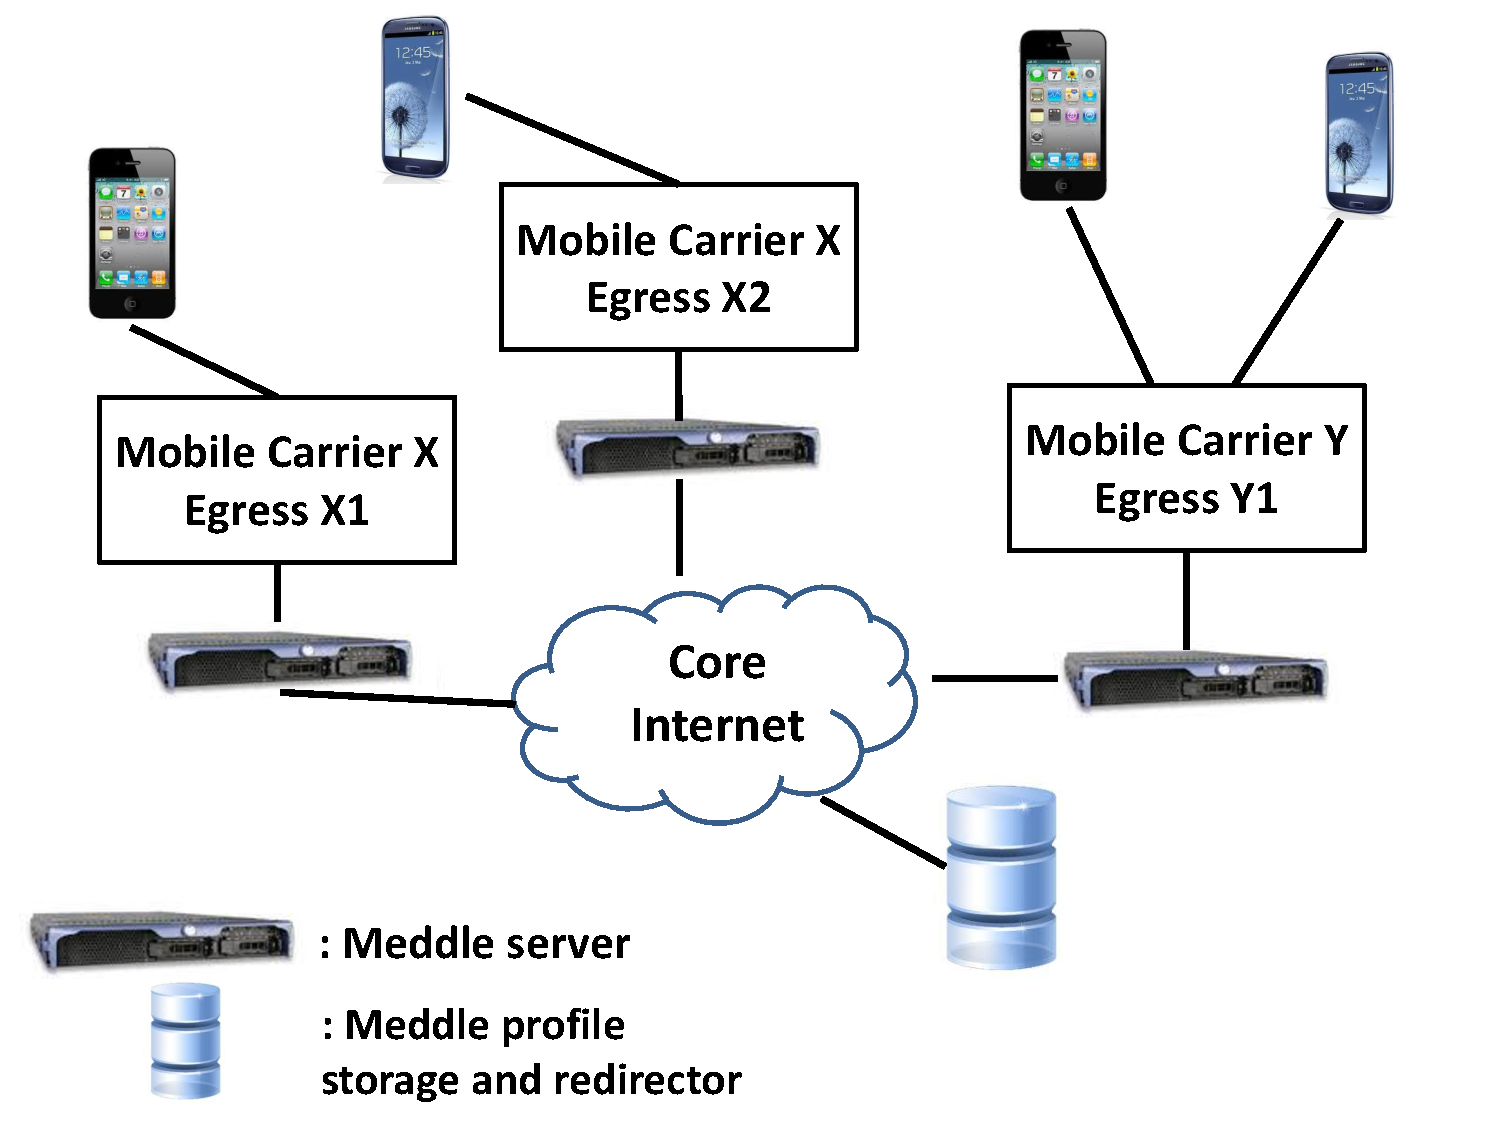
\includegraphics[width=0.8\linewidth]{figs/architecture.pdf}
\vspace{\figcapspace}
  \caption{\meddle architecture, using two carriers (X and Y) and 
  three egress points (X1 and X2 for carrier X and Y1 for carrier Y). 
  Devices are dynamically mapped to \meddle servers near each egress point, 
  and the profile manager ensures that device-specific middlebox settings 
  migrate with users as they are mapped to different \meddle servers.}
  \label{fig:arch}
\vspace{\postfigspace}
\end{figure}

%\tbd{there are typos in the figure: use Egress 1, 2 and 3, and carrier
%  X, Y, and Z}



%Because the mapping between a device and its \meddle server may change over time and as users
%travel with their devices, we would like to be able to migrate the
%custom middlebox settings with them in a platform- and
%location-independent way. 
%%Arnaud: text I removed and replaced with the text below (in \ty{})
%%Each time the redirector selects a \meddle
%%server, it instructs the {\it profile storage} to upload the middlebox
%%settings for the device on the \meddle server (assuming it is not already 
%%cached at the server).
%\ty{When the \meddle server authenticates the
%mobile device using the VPN's credentials, it downloads  the middlebox
%settings for the device from the {\it profile storage} (assuming it is not already 
%cached at the server).} The middlebox settings
%can enact content filters (ad blocking and parental controls), app
%accelerators (content caches) or custom protocols (interposing SPDY~\cite{google-spdy}).

%Arnaud: the new description is clear enough. I remove this comment
%\tbd{Arnaud: there is still a problem here. The authentication is only
%  performed at the Meddle server. Do we
%need authentication using VPN credentials at the redirector (probably yes)? Can we use one time authentication
%or delegation? This needs to be clarified.}

%The \meddle server uses the VPN credentials provided by the mobile device
%to look up the corresponding middlebox settings to load for the
%connection. For example, the server can enact content filters (ad
%blocking and parental controls), app accelerators (content caches) or
%custom protocols (interposing SPDY).
%
%The architecture of \meddle is relatively straightforward. Mobile devices establish a VPN tunnel to a \meddle server, which could run in a hosting center, on a distributed platform such as PlanetLab, EC2 or Compute Engine, or in a user's home network. The \meddle server uses the VPN credentials provided by the mobile device to look up the corresponding middlebox settings to load for the connection. For example, the server can enact content filters (ad blocking and parental controls), app accelerators (content caches) or custom protocols (interposing SPDY). 
%
%When devices connect to a \meddle server, we would like to use one that is relatively near the location at which data exits the mobile carrier's network to enter the Internet. Because this may change over time and as users travel with their devices, we would like to be able to migrate the custom middlebox settings with them in a platform- and location-independent way. We observe that the mapping between VPN hostname and the particular server it resolves to can be performed dynamically, allowing us to direct mobile devices to nearby servers similar to the Akamai CDN. Given this model, our design includes a software middlebox (e.g., Vyatta), thus simplifying a large distributed deployment and facilitating migration of device-specific middlebox settings from one \meddle server to another. 
 

%%% Local Variables: 
%%% TeX-master: "hotnets-meddle-middle.tex"
%%% End:
